\section{Мета роботи}
Закріпити знання про алгоритми пошуку, що потребують
додаткової пам’яті; набути навичок виконання операцій пошуку із
використанням таблиць прямого доступу, довідників та хешованих таблиць.

\noindent
\textbf{Теми для попередньої роботи:}
\begin{itemize}
    \item масиви та списки;
    \item файли;
    \item прості алгоритми пошуку;
    \item алгоритми пошуку із застосуванням таблиць прямого доступу;
    \item поняття про хеш-таблиці, функції хешування, колізії;
    \item алгоритми розв’язання колізій.
\end{itemize}


\section{Завдання}
Початкові дані містяться у текстовому файлі. Прочитати файл,
створити таблицю прямого доступу або хеш-таблицю відповідно до
завдання з табл. 10.1. Перевірити працездатність створених таблиць на
прикладі операцій пошуку.

Порівняти час пошуку із використанням створених таблиць та простих
алгоритмів пошуку з лабораторної роботи 4. Для кожного з алгоритмів
визначити кількість порівнянь у наборі даних з різною кількістю елементів
(20, 1000, 5000, 10000, 50000), визначити час пошуку, заповнити таблицю за
формою табл. 10.2, побудувати графіки, зробити висновки.

\begin{figure}[ht!]
    \centering
    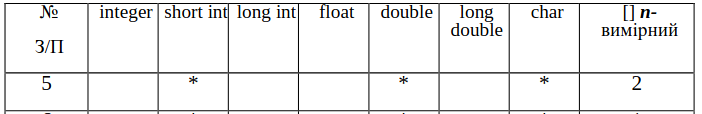
\includegraphics[width=.9\textwidth]{\assetsDirectory/var.png}
    \caption{Завдання за варіантом (\variant)}
\end{figure}


\section{Хід виконання}
Для виконання завдання було обрано мову Rust.
Увесь код також додатково був розміщений в GitHub репозитарії: \href{https://github.com/blackgolyb/algos-labs}{https://github.com/blackgolyb/algos-labs}.


\newpage
\subsection{Хеш-функція}
Розглянемо спочатку нашу функцію: функція перетворення системи числення та ділення за модулем.
Така функція буде мати дві змінні, які будуть впливати на кількість колізій - це параметр системи числення (base) та число, по якому модулю ми будемо брати,
що своєю чергою є розміром (size) нашої хеш-таблиці.
Тому перед подальшою роботою треба провести дослідження цієї функції та знайти оптимальні параметри.

Для цього напишемо програму, яка на певній рівномірно розподіленій вибірці, значення якої лежить в діапазоні $[0, 2^{63} - 1]$,
розмір вибірки візьмемо $n = 1000$ і для кожної пари $(base, size)$ будемо рахувати помилку (error) за таким алгоритмом:
\begin{enumerate}
    \item Створюємо масив розміром size
    \item Знаходимо цільову кількість елементів на кожен backet за формулою: $target = n / size$
    \item Для кожного елемента в вибірці рахуємо його хеш
    \item За знайденим хешем додаємо до масиву 1
    \item Після обробки усієї вибірки рахуємо MSE між нашим масивом та target
\end{enumerate}
Для подальшого досліду візьмемо значення base в діапазоні $[2, 257]$, а значення size в діапазоні $[8, n]$

Щоб оцінити, як функція поводить себе при різних значеннях, побудуємо графік помилки нашої функції за вище описаним алгоритмом.
Використаємо Python та бібліотеки для візуалізації для побудови цього графіку.

\begin{figure}[ht!]
    \centering
    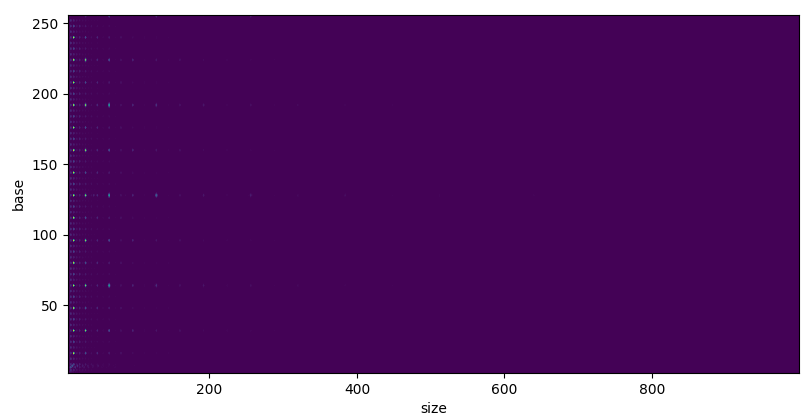
\includegraphics[width=.9\textwidth]{\assetsDirectory/viz.png}
    \caption{Графік функції помилки}
\end{figure}

\begin{figure}[ht!]
    \centering
    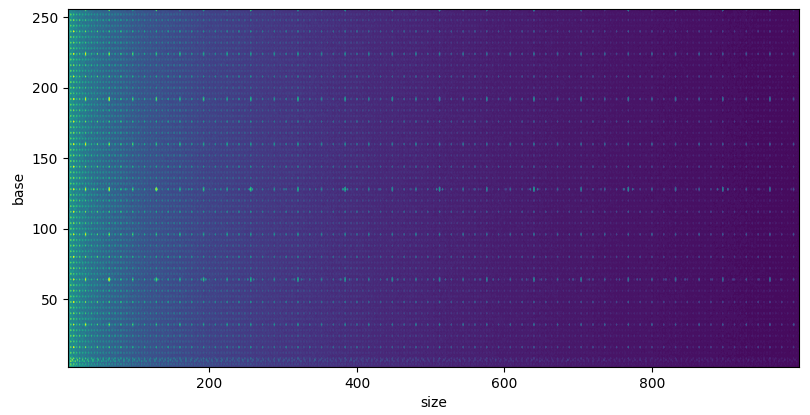
\includegraphics[width=.9\textwidth]{\assetsDirectory/viz_log.png}
    \caption{Графік функції помилки з логарифмованим значенням помилки для згладження піків}
\end{figure}

Як можна побачити з вищенаведених графіків хеш-функція за парних значень набуває більшого значення помилки,
а особливо на значеннях коли base та size є ступенем двійки. Також в ході дослідження було знайдено,
що найкраще себе показує функція коли значення base та size є простими,
але різниця не настільки суттєва якщо порівнювати з непарними числами.
Тому надалі для обрання параметрів base та size будемо використовувати непарні числа.

Також хочеться зазначити, що таку хеш-функцію краще не використовувати в реальній роботі,
бо вона: повільно працює, дуже перебірлива до вхідних параметрів та не підходить до будь-яких даних.
Тому на цей час найкращий вибір буде \href{https://github.com/Cyan4973/xxHash}{xxHash}, бо вона:
працює на граничній швидкості оперативної пам'яті,
дає дуже гарний розподіл хешу та
працює не представленням даних, а з набором байтів.


\newpage
\subsection{Хеш-таблиця}
Реалізуємо хеш-таблицю де ключем може бути будь-який тип який можна хешувати та порівняти, а значенням будь-який тип.
\lstinputlisting[language=Rust, style=colouredRust]{\codeDirectory/src/libs/hash_table/lib.rs}


\newpage
\subsection{Опис даних}
Напишемо структуру даних як описана у завданні та напишемо для неї серіалі затор та десереалізатор.
А також функції для генерації випадкових значень цих даних.
\lstinputlisting[language=Rust, style=colouredRust]{\codeDirectory/src/labs/lab10/data.rs}

\begin{figure}[ht!]
    \centering
    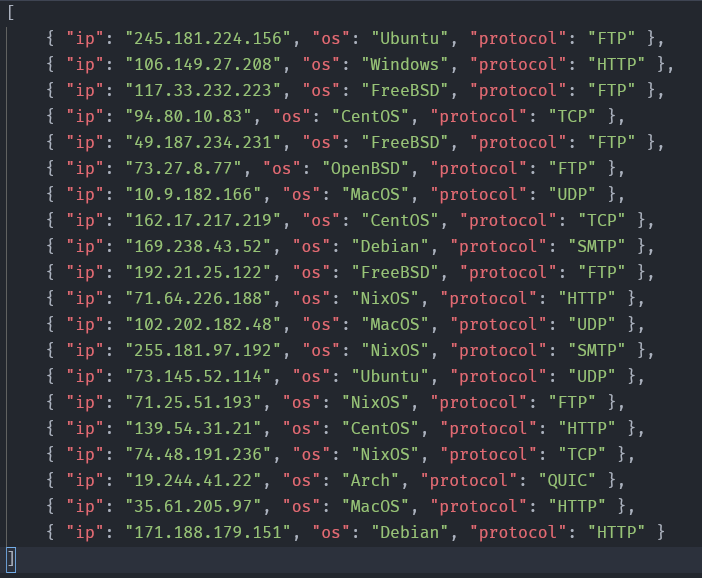
\includegraphics[width=.8\textwidth]{\assetsDirectory/data.png}
    \caption{Приклад збережених даних}
\end{figure}

\newpage
\subsection{Приклад роботи програми}
Для перевірки працездатності напишемо програму, яка буде порівнювати хеш-таблицю, двійковий та лінійний пошук у лінійному списку.
А також програму для виводу вмісту таблиці.

\noindent
Код програми для перевірки:
\lstinputlisting[language=Rust, style=colouredRust]{\codeDirectory/src/labs/lab10/main.rs}


\begin{figure}[ht!]
    \centering
    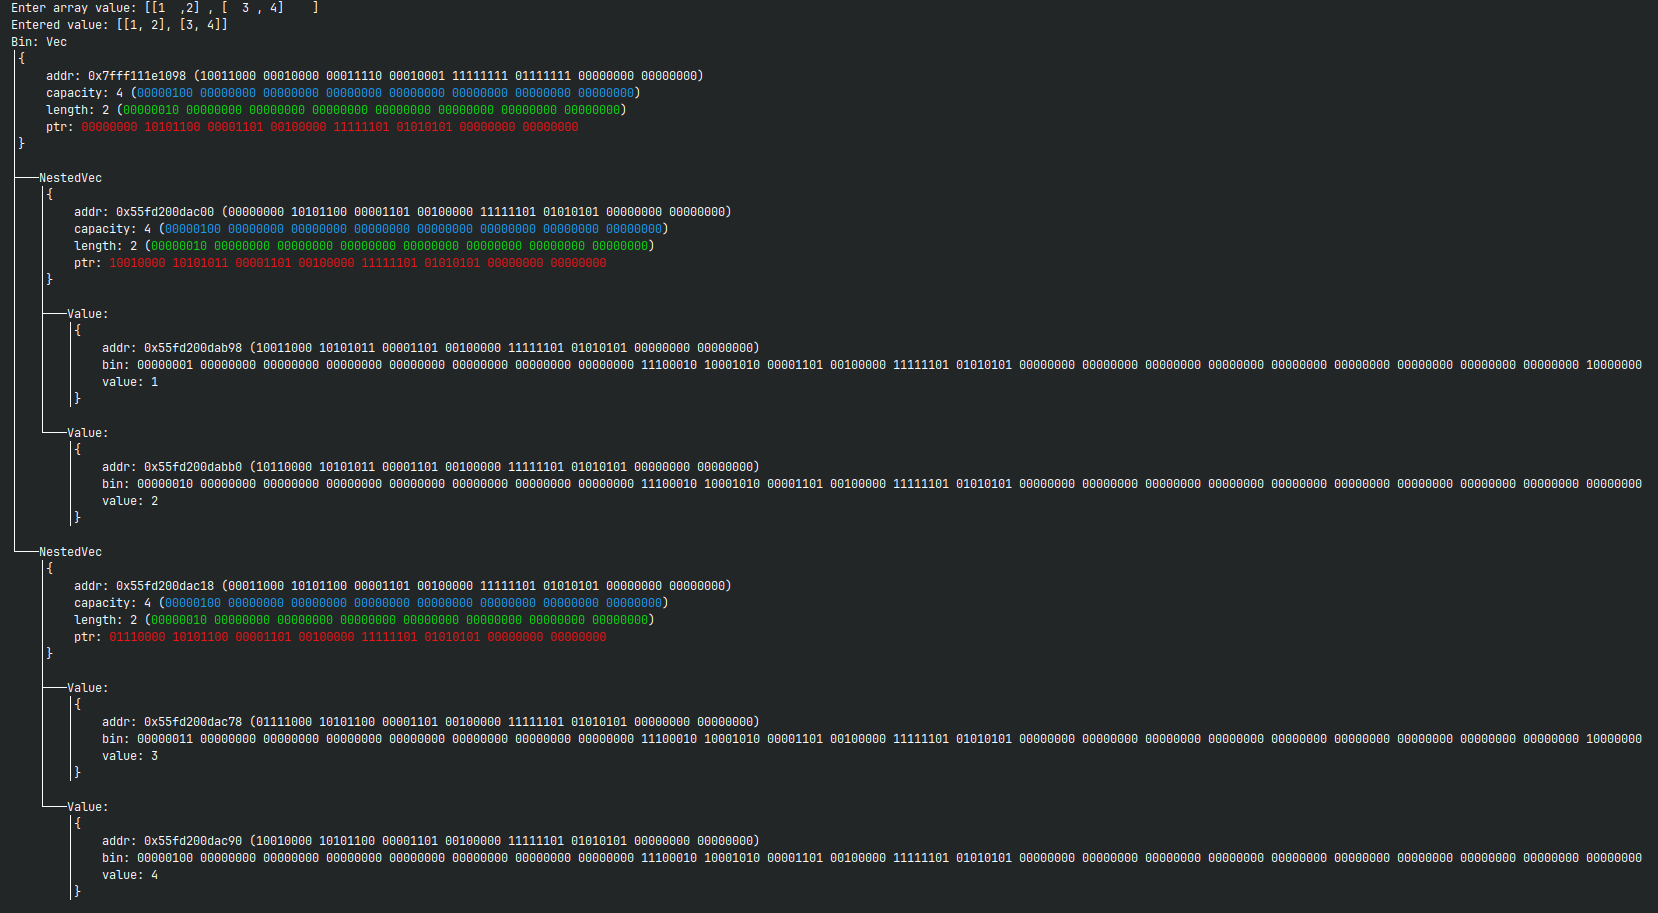
\includegraphics[width=.8\textwidth]{\assetsDirectory/res.png}
    \caption{Приклад роботи}
\end{figure}

\begin{figure}[ht!]
    \centering
    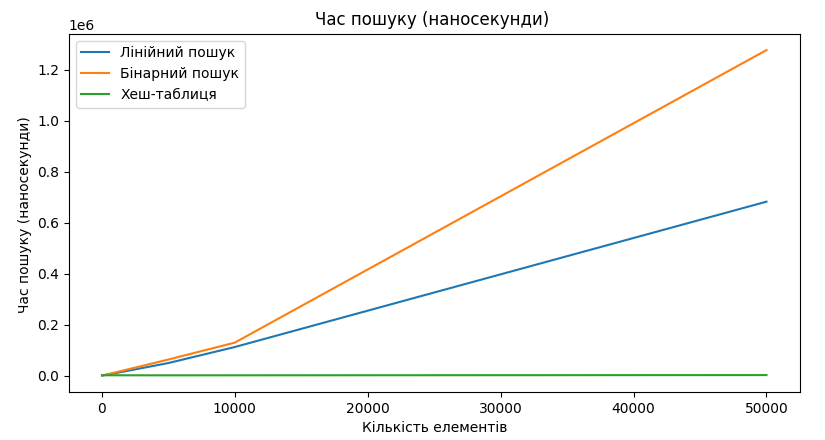
\includegraphics[width=.8\textwidth]{\assetsDirectory/time.png}
    \caption{Залежність часу пошуку від кількості елементів}
\end{figure}
\begin{figure}[ht!]
    \centering
    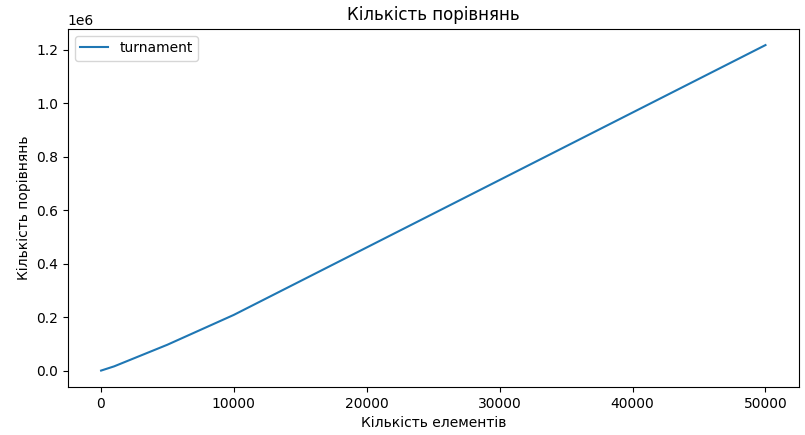
\includegraphics[width=.8\textwidth]{\assetsDirectory/comp.png}
    \caption{Залежність кількості порівнянь від кількості елементів}
\end{figure}


\newpage
\section{Висновки}
В ході виконання лабораторної робити було створено хеш-таблицю.
Також було порівняно хеш-таблицю з лінійним та бінарним пошуком в списку.
За результатами порівняння було виявлено, що хеш-таблиця набагато ефективніше за інші способи
а також вона не потребує відсортований набір даних як бінарний пошук.
